\begin{figure}[htb]
    \centering
    \caption{Modelo de domínio simplificado da aplicação}
    \label{fig:modelo-dominio}
    \resizebox{\textwidth}{!}{%
    \newcommand*{\titent}[1]{{\small\bfseries #1\strut}\par\vspace{1pt}\hrule\vspace{3pt}}%
    \newcommand*{\atr}[1]{\par\hangindent=0.9em\hangafter=1\noindent\makebox[0.9em][l]{\textbullet}#1\par}%
    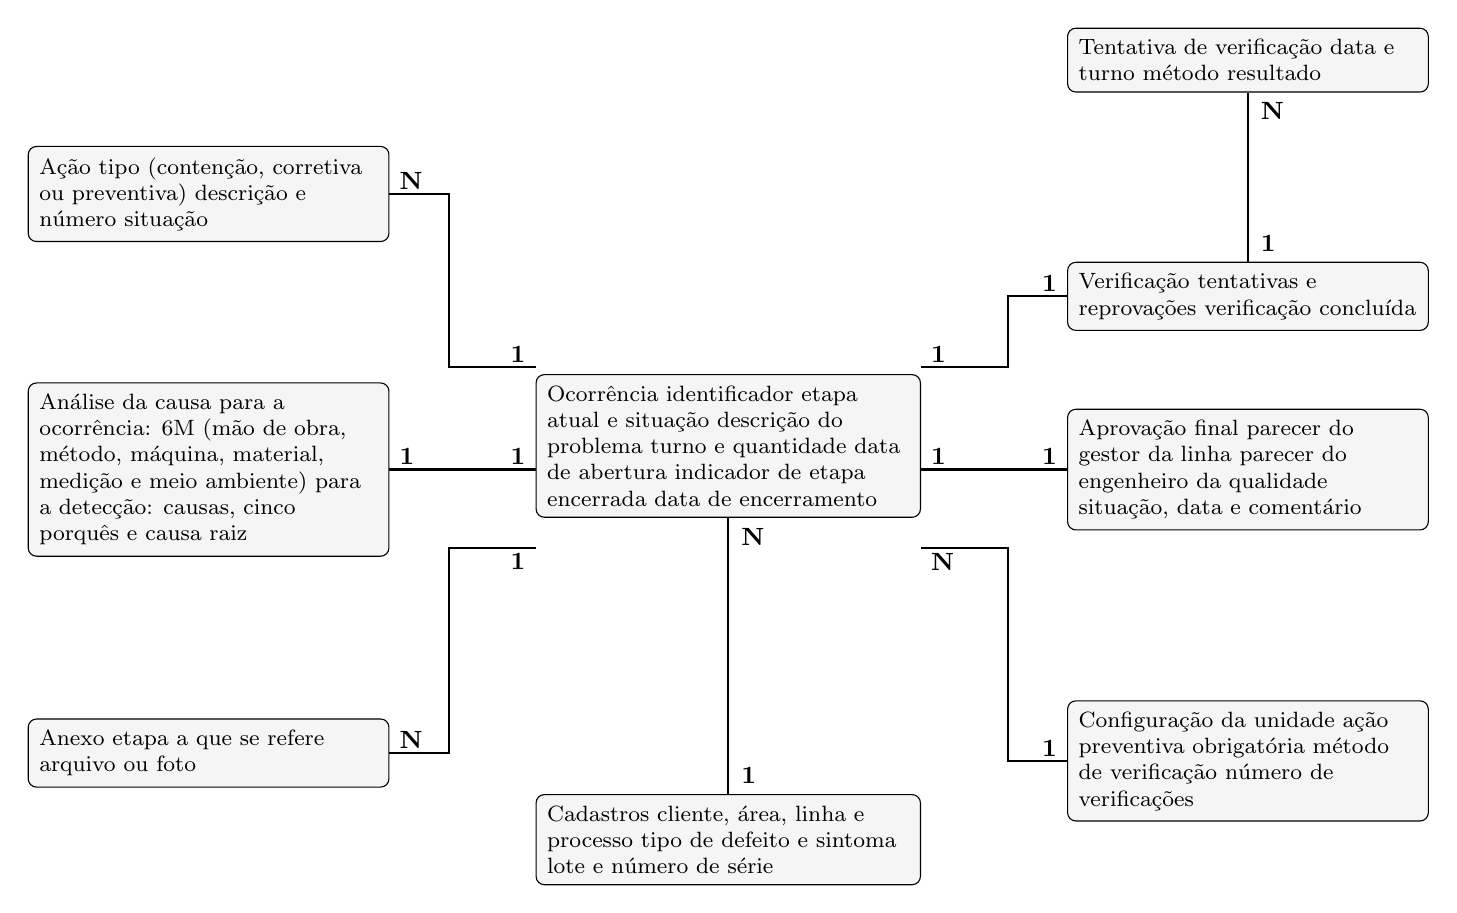
\begin{tikzpicture}[
        ent/.style={draw, rounded corners=3pt, fill=gray!8, align=flush left,
            inner sep=4pt, font=\footnotesize, text width=4.3cm},
        lig/.style={thick},
        card/.style={font=\small\bfseries, inner sep=1.5pt}
    ]
    \node[ent, text width=4.6cm] (oc) at (0,0) {%
        \titent{Ocorrência}
        \atr{identificador}
        \atr{etapa atual e situação}
        \atr{descrição do problema}
        \atr{turno e quantidade}
        \atr{data de abertura}
        \atr{indicador de etapa encerrada}
        \atr{data de encerramento}};

    \node[ent] (acao) at (-6.6,3.2) {%
        \titent{Ação}
        \atr{tipo (contenção, corretiva ou preventiva)}
        \atr{descrição e número}
        \atr{situação}};
    \node[ent] (causa) at (-6.6,-0.3) {%
        \titent{Análise da causa}
        \atr{para a ocorrência: 6M (mão de obra, método, máquina, material, medição e meio ambiente)}
        \atr{para a detecção: causas, cinco porquês e causa raiz}};
    \node[ent] (anexo) at (-6.6,-3.9) {%
        \titent{Anexo}
        \atr{etapa a que se refere}
        \atr{arquivo ou foto}};

    \node[ent] (verif) at (6.6,1.9) {%
        \titent{Verificação}
        \atr{tentativas e reprovações}
        \atr{verificação concluída}};
    \node[ent] (tent) at (6.6,4.9) {%
        \titent{Tentativa de verificação}
        \atr{data e turno}
        \atr{método}
        \atr{resultado}};
    \node[ent] (aprov) at (6.6,-0.3) {%
        \titent{Aprovação final}
        \atr{parecer do gestor da linha}
        \atr{parecer do engenheiro da qualidade}
        \atr{situação, data e comentário}};
    \node[ent] (conf) at (6.6,-4.0) {%
        \titent{Configuração da unidade}
        \atr{ação preventiva obrigatória}
        \atr{método de verificação}
        \atr{número de verificações}};

    \node[ent, text width=4.6cm] (cad) at (0,-5.0) {%
        \titent{Cadastros}
        \atr{cliente, área, linha e processo}
        \atr{tipo de defeito e sintoma}
        \atr{lote e número de série}};

    % Ligações ortogonais; a cardinalidade fica junto à entidade a que se refere
    \def\xl{-3.55}\def\xr{3.55}
    % Ocorrência 1 -- N Ação
    \draw[lig] ([yshift=1.0cm]oc.west) -| (\xl,0 |- acao.east) -- (acao.east);
    \node[card, anchor=south east] at ([xshift=-2pt,yshift=1.0cm]oc.west) {1};
    \node[card, anchor=south west] at ([xshift=2pt]acao.east) {N};
    % Ocorrência 1 -- 1 Análise da causa
    \draw[lig] (oc.west |- causa.east) -- (causa.east);
    \node[card, anchor=south east] at ([xshift=-2pt]oc.west |- causa.east) {1};
    \node[card, anchor=south west] at ([xshift=2pt]causa.east) {1};
    % Ocorrência 1 -- N Anexo
    \draw[lig] ([yshift=-1.3cm]oc.west) -| (\xl,0 |- anexo.east) -- (anexo.east);
    \node[card, anchor=north east] at ([xshift=-2pt,yshift=-1.3cm]oc.west) {1};
    \node[card, anchor=south west] at ([xshift=2pt]anexo.east) {N};
    % Ocorrência 1 -- 1 Verificação
    \draw[lig] ([yshift=1.0cm]oc.east) -| (\xr,0 |- verif.west) -- (verif.west);
    \node[card, anchor=south west] at ([xshift=2pt,yshift=1.0cm]oc.east) {1};
    \node[card, anchor=south east] at ([xshift=-2pt]verif.west) {1};
    % Verificação 1 -- N Tentativa de verificação
    \draw[lig] (verif.north) -- (tent.south);
    \node[card, anchor=south west] at ([xshift=3pt,yshift=2pt]verif.north) {1};
    \node[card, anchor=north west] at ([xshift=3pt,yshift=-2pt]tent.south) {N};
    % Ocorrência 1 -- 1 Aprovação final
    \draw[lig] (oc.east |- aprov.west) -- (aprov.west);
    \node[card, anchor=south west] at ([xshift=2pt]oc.east |- aprov.west) {1};
    \node[card, anchor=south east] at ([xshift=-2pt]aprov.west) {1};
    % Ocorrência N -- 1 Configuração da unidade
    \draw[lig] ([yshift=-1.3cm]oc.east) -| (\xr,0 |- conf.west) -- (conf.west);
    \node[card, anchor=north west] at ([xshift=2pt,yshift=-1.3cm]oc.east) {N};
    \node[card, anchor=south east] at ([xshift=-2pt]conf.west) {1};
    % Ocorrência N -- 1 Cadastros
    \draw[lig] (oc.south) -- (cad.north);
    \node[card, anchor=north west] at ([xshift=3pt,yshift=-2pt]oc.south) {N};
    \node[card, anchor=south west] at ([xshift=3pt,yshift=2pt]cad.north) {1};
    \end{tikzpicture}}
    \legend{Fonte: elaborado pelo autor (2026), com base no modelo de domínio da aplicação.}
\end{figure}
